% !TeX document-id = {631e44a8-cd91-47da-bf82-1571f8787194}
% !TeX TXS-program:compile = txs:///pdflatex/[--shell-escape]

\documentclass{class/thesis}

%%%%%%%%%%%%%%%%%%%%%%%%%%%%%%%%%%%%%%%%%%%%%%%%%%%%%%%%%%%%
% Bitte ergänzen Sie Ihre persönlichen Daten innerhalb     %
% der im Folgenden inkludierten Datei properties.tex       %
%%%%%%%%%%%%%%%%%%%%%%%%%%%%%%%%%%%%%%%%%%%%%%%%%%%%%%%%%%%%

%%%%%%%%%%%%%%%%%%%%%%%%%%%%%%%%%%%%%%%%%%%%%%%%
% Titel der Arbeit                             %
%%%%%%%%%%%%%%%%%%%%%%%%%%%%%%%%%%%%%%%%%%%%%%%%
\thesistitle{Entwicklung eines Log-strukturierten Heaps für NVRAM}

%%%%%%%%%%%%%%%%%%%%%%%%%%%%%%%%%%%%%%%%%%%%%%%%
% Schlüsselwörter                              %
%%%%%%%%%%%%%%%%%%%%%%%%%%%%%%%%%%%%%%%%%%%%%%%%
\thesiskeywords{NVRAM, Log-strukturiert, Log-Struktur, Heap}

%%%%%%%%%%%%%%%%%%%%%%%%%%%%%%%%%%%%%%%%%%%%%%%%
% Sprache der Arbeit                           %
%                                              %
%   ngerman  - Deutsch (neue Rechtschreibung)  %
%   english  - Englisch                        %
%%%%%%%%%%%%%%%%%%%%%%%%%%%%%%%%%%%%%%%%%%%%%%%%
\thesislanguage{ngerman}

%%%%%%%%%%%%%%%%%%%%%%%%%%%%%%%%%%%%%%%%%%%%%%%%
% Art der Arbeit                               %
%                                              %
%   bachelor  - Bachelorarbeit                 %
%   master    - Masterarbeit                   %
%   project   - Projektarbeit                  %
%%%%%%%%%%%%%%%%%%%%%%%%%%%%%%%%%%%%%%%%%%%%%%%%
\thesistype{bachelor}

%%%%%%%%%%%%%%%%%%%%%%%%%%%%%%%%%%%%%%%%%%%%%%%%
% Ausgabe von Verzeichnissen                   %
%                                              %
%   true   - Aktiviert                         %
%   false  - Deaktiviert                       %
%%%%%%%%%%%%%%%%%%%%%%%%%%%%%%%%%%%%%%%%%%%%%%%%
\listofalgorithmsenabled{true}
\listoffiguresenabled{true}
\listoftablesenabled{true}

%%%%%%%%%%%%%%%%%%%%%%%%%%%%%%%%%%%%%%%%%%%%%%%%
% Vollständiger Name                           %
%%%%%%%%%%%%%%%%%%%%%%%%%%%%%%%%%%%%%%%%%%%%%%%%
\thesisauthor{Maximilian Vogel}

%%%%%%%%%%%%%%%%%%%%%%%%%%%%%%%%%%%%%%%%%%%%%%%%
% Geburtsort                                   %
%%%%%%%%%%%%%%%%%%%%%%%%%%%%%%%%%%%%%%%%%%%%%%%%
\authorbirthplace{Wuppertal}

%%%%%%%%%%%%%%%%%%%%%%%%%%%%%%%%%%%%%%%%%%%%%%%%
% Datum der Abgabe                             %
%%%%%%%%%%%%%%%%%%%%%%%%%%%%%%%%%%%%%%%%%%%%%%%%
\submissiondate{21. September 2023}

%%%%%%%%%%%%%%%%%%%%%%%%%%%%%%%%%%%%%%%%%%%%%%%%
% Erstgutachter                                %
%%%%%%%%%%%%%%%%%%%%%%%%%%%%%%%%%%%%%%%%%%%%%%%%
\firstreviewer{Prof. Dr. Michael Schöttner}

%%%%%%%%%%%%%%%%%%%%%%%%%%%%%%%%%%%%%%%%%%%%%%%%
% Zweitgutachter                               %
%%%%%%%%%%%%%%%%%%%%%%%%%%%%%%%%%%%%%%%%%%%%%%%%
\secondreviewer{Prof. Dr. Stefan Conrad}

%%%%%%%%%%%%%%%%%%%%%%%%%%%%%%%%%%%%%%%%%%%%%%%%
% Betreuer                                     %
%%%%%%%%%%%%%%%%%%%%%%%%%%%%%%%%%%%%%%%%%%%%%%%%
\supervisor{Prof. Dr. Michael Schöttner}

\begin{document}

  \begin{thesis}

    %%%%%%%%%%%%%%%%%%%%%%%%%%%%%%%%%%%%%%%%%%%%%%%%%%%%%%%%%%%%%%%%%
    % Die folgenden Kapitel dienen lediglich als Hilfestellung      %
    % und müssen somit mit der Fertigstellung des finalen Dokuments %
    % unbedingt entfernt werden.                                    %
    %%%%%%%%%%%%%%%%%%%%%%%%%%%%%%%%%%%%%%%%%%%%%%%%%%%%%%%%%%%%%%%%%

%    \include{chap/einleitung}
%    \include{chap/gliederung}
%    \include{chap/struktur}
%    \include{chap/organisation}
%    \include{chap/text}
%    \include{chap/zitieren}
%    \include{chap/auflistungen}
%    \include{chap/bilder}
%    \include{chap/tabellen}
%    \include{chap/matheumgebung}
%    \include{chap/code}

	\chapter{Einleitung}
	
	
	

	\chapter{Grundlagen}
	
	\section{Was ist NVRAM}
	NVRAM ist die Abkürzung für \glqq{}Non Volatile Random Access Memory\grqq{}, also nicht flüchtiger Hauptspeicher. Eine andere häufig genutzte Bezeichnung ist \glqq{}Persistent Memory\grqq{}.
	Wie in Abbildung \ref{bildSpeicherHierarchie} zu sehen ist, ordnet sich NVRAM in der Speicher Hierarchie zwischen DRAM und SSDs ein und vereint somit die Vorteile von DRAM und Sekundärspeicher.
	
	\begin{figure}[h]
		\centering
		\begin{subfigure}[b]{1.0\textwidth}
			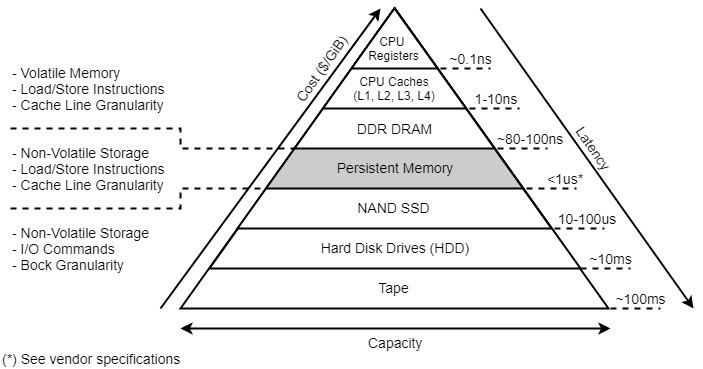
\includegraphics[width=1.0\linewidth]{img/pmem_storage_pyramid}
		\end{subfigure}
		\caption{Speicher Hierarchie \cite{PMEM.IO}}
		\label{bildSpeicherHierarchie}
	\end{figure}
	
	NVRAM ist im Gegensatz zu DRAM, wie der Name schon sagt, persistent. Somit bleiben die Daten im Speicher erhalten, wenn der Computer, sei es bewusst oder z.B. durch einen Stromausfall, ausgeschaltet wird und sind  nach dem Systemstart direkt wieder nutzbar, ohne dass sie erst vom Sekundärspeicher geladen werden müssen \cite{Scargall:2020:PPM}.
	Die Geschwindigkeit von NVRAM kommt zwar nicht ganz an die von DRAM heran, ist aber trotzdem um ein vielfaches schneller, als die von SSDs \cite{PMEM.IO}.
	Die Speicherkapazität und der Preis ordnen sich ebenfalls entsprechend zwischen DRAM und SSDs ein \cite{PMEM.IO} und die Lebensdauer von NVRAM ist länger, als die von SSDs \cite{Scargall:2020:PPM}. \\
	Außerdem ist NVRAM Byte adressierbar und es können per \glqq{}Direct Access\grqq{}(DAX) direkt Load und Store Instruktionen ausgeführt werden, ohne Code aus dem Kernel zu verwenden \cite{Rudoff:2017:PMP}. 
	Das bringt folgenden Vorteil: Angenommen ich möchten 8 Byte in meinen Daten ändern, dann kann ich, wenn die Daten im NVRAM liegen, diese 8 Byte direkt schreiben. Wenn die Daten jedoch im Sekundärspeicher liegen, muss erst der entsprechende Block geladen werden, dieser ist meist 4 KB groß. Dann können die Daten aktualisiert werden und anschließend muss der Block wieder in den Sekundärspeicher geschrieben werden \cite{Scargall:2020:PPM}. \\
	Da NVRAM persistent ist, müssen die Daten im Speicher wiedergefunden werden können und können nicht wie bei DRAM anonym sein. Um das zu erreichen wird die selbe Semantik, wie bei Dateien im Sekundärspeicher verwendet. Die Daten werden mit den Standardbefehlen gemappt und haben einen Namen, sowie Zugriffsrechte. Nachdem sie gemappt wurden, kann per DAX auf sie zugegriffen werden \cite{Rudoff:2017:PMP}. Es ist wichtig zu beachten, dass es nicht alleine ausreicht Daten per Store Instruktion zu schreiben, sondern man auch die Caches flushen muss, andernfalls sind sie nicht persistiert und könnten verloren gehen \cite{Rudoff:2017:PMP}.
	\todo[inline]{Reihenfolge und (8 Byte Atomarität bei Stromausfall)}
	
	
	
	\section{Wie sieht Log-strukturierter Speicher aus}
	
	In einem Log-strukturierten Speicher werden neue Daten einfach an das Ende des Logs angehangen, dadurch spart man sich die Zeit zuerst eine passende Stelle finden zu müssen. Klassisch strukturierte Speicher benutzten zwar auch Logs, allerdings werden die Daten dort nur temporär gespeichert und anschließend an den richtigen Speicherplatz geschrieben. Die Daten müssen also, im Gegensatz zu Log-strukturiertem Speicher, zwei mal geschrieben werden, bevor sie persistiert sind \cite{Rosenblum:1992}.
	Da das Log unveränderlich ist können Daten in ihm nicht aktualisiert werden, das hat die Folge, dass aktualisierte Daten neu an das Log angehangen werden müssen. Alte Versionen der Daten müssen also entfernt werden, um keinen Speicherplatz zu verschwenden. Die durch das Löschen der Daten entstehenden Lücken können allerdings nicht genutzt werden, da neue Daten immer nur am Ende des Logs eingefügt werden.
	Dieses Problem löst der Cleaner. \\
	Der Cleaner hat zwei Aufgaben. Die erste ist das Löschen von Daten und das finden veralterter Versionen inklusive anschließendem Löschen. Die zweite ist das Kompaktieren des Logs, wodurch freie Stellen im Log wieder benutzt werden können. \\
	In der Regel wird das Log in Segmente unterteilt. Wenn ein Segment mit Daten vollgeschrieben wurde wird das nächste beschrieben. Der Cleaner kompaktiert das Log, indem er die Segmente durchgeht und noch aktuelle Daten in ein neues leeres Segment kopiert und dieses wieder in das Log einfügt. Das gesäuberte Segment steht jetzt wieder für neue Daten zur Verfügung. \\
	Welche Segmente der Cleaner zum kompaktieren auswählt und wie er die noch aktuellen Daten sortiert und wieder in das Log einfügt ist eine Frage der Implementierung und kann starke Auswirkungen auf die gesamte Performance haben.
	
	
	
	\section{Warum Log-strukturiert}
	
	Ein Problem in der Speicherverwaltung ist die Fragmentierung des Speichers, wodurch Speicherplatz \glqq{}verloren\grqq{} geht, indem er nicht mehr genutzt werden kann. Dabei unterscheidet man zwischen zwei Fällen.
	Bei der internen Fragmentierung verbrauchen allozierte Daten nicht nur ihre tatsächliche Größe, sondern ein vielfaches der kleinstmöglichen Speicherblockgröße im System. Wenn ein System z.b. 32 Byte große Speicherblöcke hat und 33 Byte Speicherplatz alloziert werden sollen, werden trotzdem 64 Byte alloziert und es entsteht somit ein Speicherverschnitt von 31 Byte, welcher nicht genutzt werden kann.
	Externe Fragmentierung tritt auf, wenn Speicherplatz freigegeben wird. Dabei entstehen Lücken im Speicher, welche zwar genutzt werden können, allerdings nur von Daten, die auch in die Lücke hinein passen. Wenn es also viele kleine freie Stellen im Speicher gibt, ist zwar noch einiges an freiem Speicherplatz vorhanden, dieser ist aber praktisch nicht nutzbar, sofern die zu speichernden Daten nicht klein genug sind, um hineinzupassen.\\
	Allokatoren, die im Stil von DRAM an beliebigen Stellen Speicher allozieren können, können eine Speicherfragmentierung von über 50\% erreichen \cite{Rumble:FAST14}. Das stellt für NVRAM ein besonders großes Problem dar, da die Fragmentierung im Gegensatz zu DRAM auch über den Systemneustart hinaus erhalten bleibt.
	Log-strukturierter Speicher verhindert interne Fragmentierung durch das einfache Anhängen der Daten an das Ende des Logs. Und externe Fragmentierung durch das Kompaktieren des Speichers durch den Cleaner \cite{HU:ATC17}. 
	Dadurch kann Log-strukturierter Speicher eine Speicherauslastung von 80-90\% erreichen, ohne dabei Einbuße der Performance zu haben \cite{Rumble:FAST14}. 


	
	\chapter{Implementation}




	\chapter{Evaluation}





  \end{thesis}

\end{document}

